\chapter{Group Theory and Special Relativity}
\label{chp:group theory}
Group theory concerns the classification of mathematical similarities between sets of elements and connects these to physical symmetries. 
\paragraph{Definition of a group: }
A set of elements, $a,b,c,...\in G$, is said to form a group if there, between two arbitrary elements of the group, exists a well defined product that satisfies:
\begin{enumerate}
	\item The product of two elements of the group is another element the group $a\cdot b=c$, $\forall a,b:\ni c:a,b,c\in G$.
	\item The group product between several elements is associative, i.e. $a\cdot(b\cdot c)=(a\cdot b)\cdot c$, $\forall a,b,c\in G$.
	\item The identity element exists within the group, i.e. $e\in G$. The identity is defined by the operation on other, generic elements via $a\cdot e=e\cdot a=a$, $\forall a\in G, e\in G$.
	\item There is an inverse to each group element, such that $a^{-1}\cdot a=a\cdot a^{-1}=e$, $\forall a\in G, e\in G$.
\end{enumerate}
\paragraph{An abelian group: }
A group is said to be abelian if the product of group elements is commutative, i.e. $a\cdot b=b\cdot a$, $\forall a,b\in G$.
\paragraph{Order of a group: }
The order of a group is the number of elements in the group.
\paragraph{Subgroup: }
If a subset, $H$, of a group, $G$, fulfill the requirements for a group, then the subset forms a subgroup.
\paragraph{Continuous group: }
If the group elements carry a label, which is a continuous parameter, the group is said to be continuous. A continuous group of special interest to physics is the Lie group\index{Lie group}. A Lie group is a group which is also a differentiable manifold\index{Manifold}. In mathematics, a manifold is a topological space that locally resembles Euclidean space near each point. This means that a geometrical structure can be associated with Lie groups and the group can be associated with such a structure in some abstract space. Further more, the elements of a Lie group must be parameterized smoothly and continuously.
\begin{example}
	\begin{enumerate}
		\item The general linear group, of dimension $n$, $GL(n)$, can be represented as the set of all invertible $n\times n$ matrices.
		\item The unitary group, of dimension $n$, $U(n)$, can be represented as the set of $n\times n$ unitary matrices. Ie. matrices satisfying $UU^\dagger=U^\dagger U=I$.
		\item The special unitary group, of dimension $n$, $SU(n)$, can be represented as the set of unitary matrices with unit determinant.
		\item The orthogonal group, of dimension $n$, $O(n)$, can be represented as the set of real, orthogonal matrices. Ie. matrices satisfying $M^T=M^{-1}$. The different groups are connected via the relation
		\begin{equation}
			SU(n)\wedge O(n)\in U(n)\in GL(n).
		\end{equation} 
		The relationship is also seen illustrated in figure \ref{fig:2}.
		\begin{figure}[h]
			\captionsetup{width=1\textwidth}
			\centering
			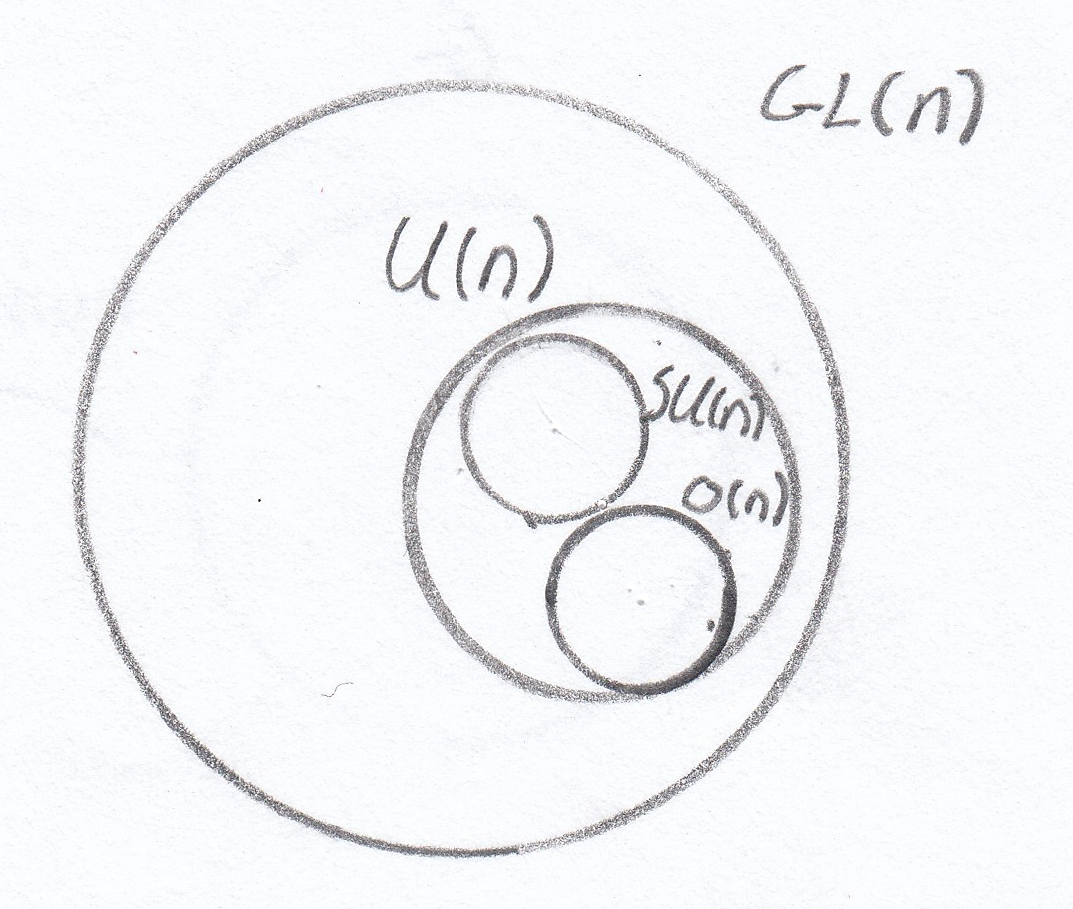
\includegraphics[width=0.4\textwidth]{figures/2}
			\caption{The relationship between the different groups mentioned above.}
			\label{fig:2}
		\end{figure}
	\end{enumerate}
\end{example}

\paragraph{Homomorphism: }
A homomorphism is a mapping between two groups, $G$ and $G'$, that conserve group multiplication. The map does not have to be one-to-one. An illustration of the mapping is seen in figure \ref{fig:3}.
\begin{figure}[h]
	\captionsetup{width=1\textwidth}
	\centering
	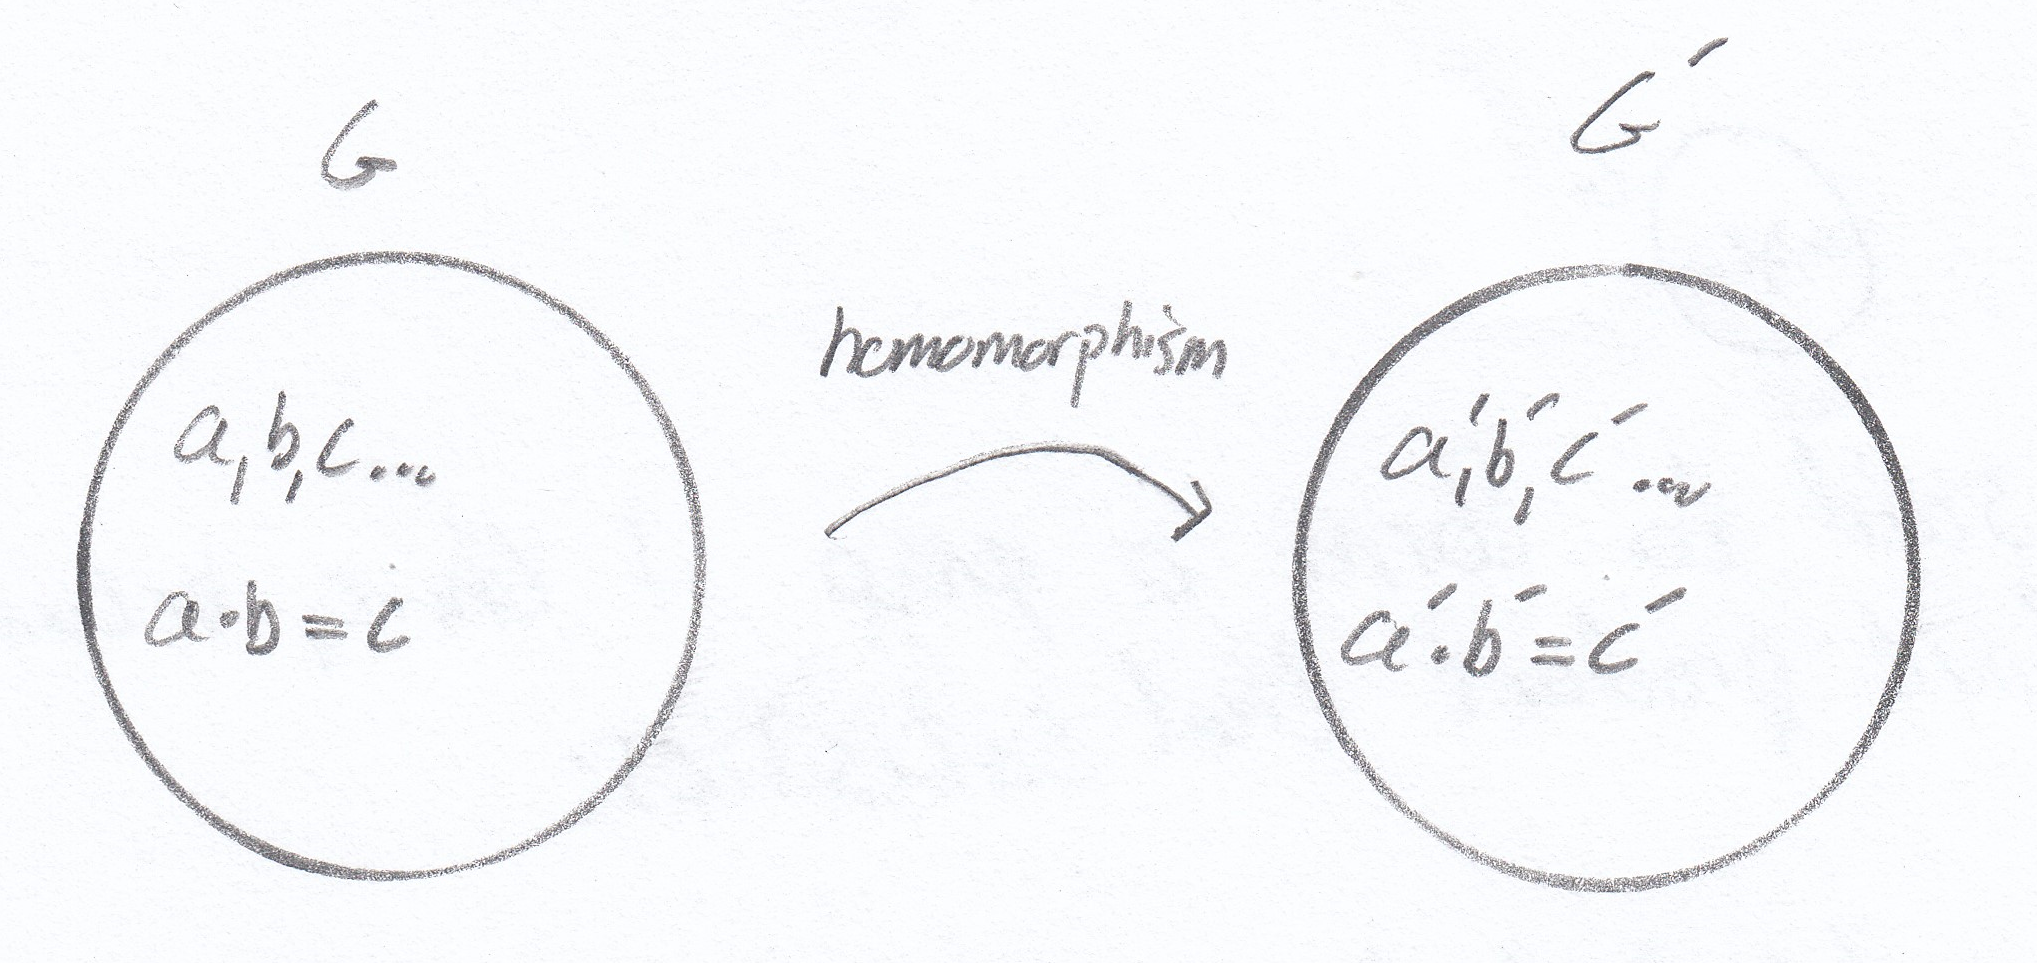
\includegraphics[width=0.5\textwidth]{figures/3}
	\caption{An illustration of a homomorphism between two groups.}
	\label{fig:3}
\end{figure}

\paragraph{Isomorphism: }
An isomorphism is a homomorphism between two groups, $G$ and $G'$, with a one-to-one correspondence. Hence, not only group multiplication is preserved, but also
\begin{equation}
	a \rightleftarrows a', \quad b \rightleftarrows b', \quad  c \rightleftarrows c',...
\end{equation}  
\paragraph{Conjugate elements of a group: }
Elements of a group, $G$, $a,b\in G$, is said to be conjugate to each other if there exist another element, $p\in G$, such that $b=pap^{-1}$.
\paragraph{Direct product group: }
Let $H_1$ and $H_2$ be subgroups of $G$ which satisfies:
\begin{enumerate}
	\item All elements of $H_1$ and $H_2$ commute, i.e. $h_1h_2=h_2h_1$, $\forall h\in H_1 \wedge h_2\in H_2$.
	\item All elements of $G$ can be described as the product of an element from $H_1$ and an element from $H_2$. Ie. $h_1h_2=g\in G, \forall g$. 
\end{enumerate}
In this case $G$ is said to be the direct product of $H_1$ and $H_2$. This is denoted by $G=H_1\otimes H_2$.
\paragraph{Group representation: }
If there is a homomorphism\footnote{A homomorphic representation is called unfaithful whereas an isomorphic representation is called faithful.} from a group, $G$, to a set of operators, $U(g)$ (where $g$ are the group elements of $G$), defined on a linear vector space, $V$, then $U(g)$ is a representation\footnote{Informally the representation of a group is a way of writing the group as matrices.} of $G$. The concept of a representation is shown in figure \ref{fig:4}.
\begin{figure}[h]
	\captionsetup{width=1\textwidth}
	\centering
	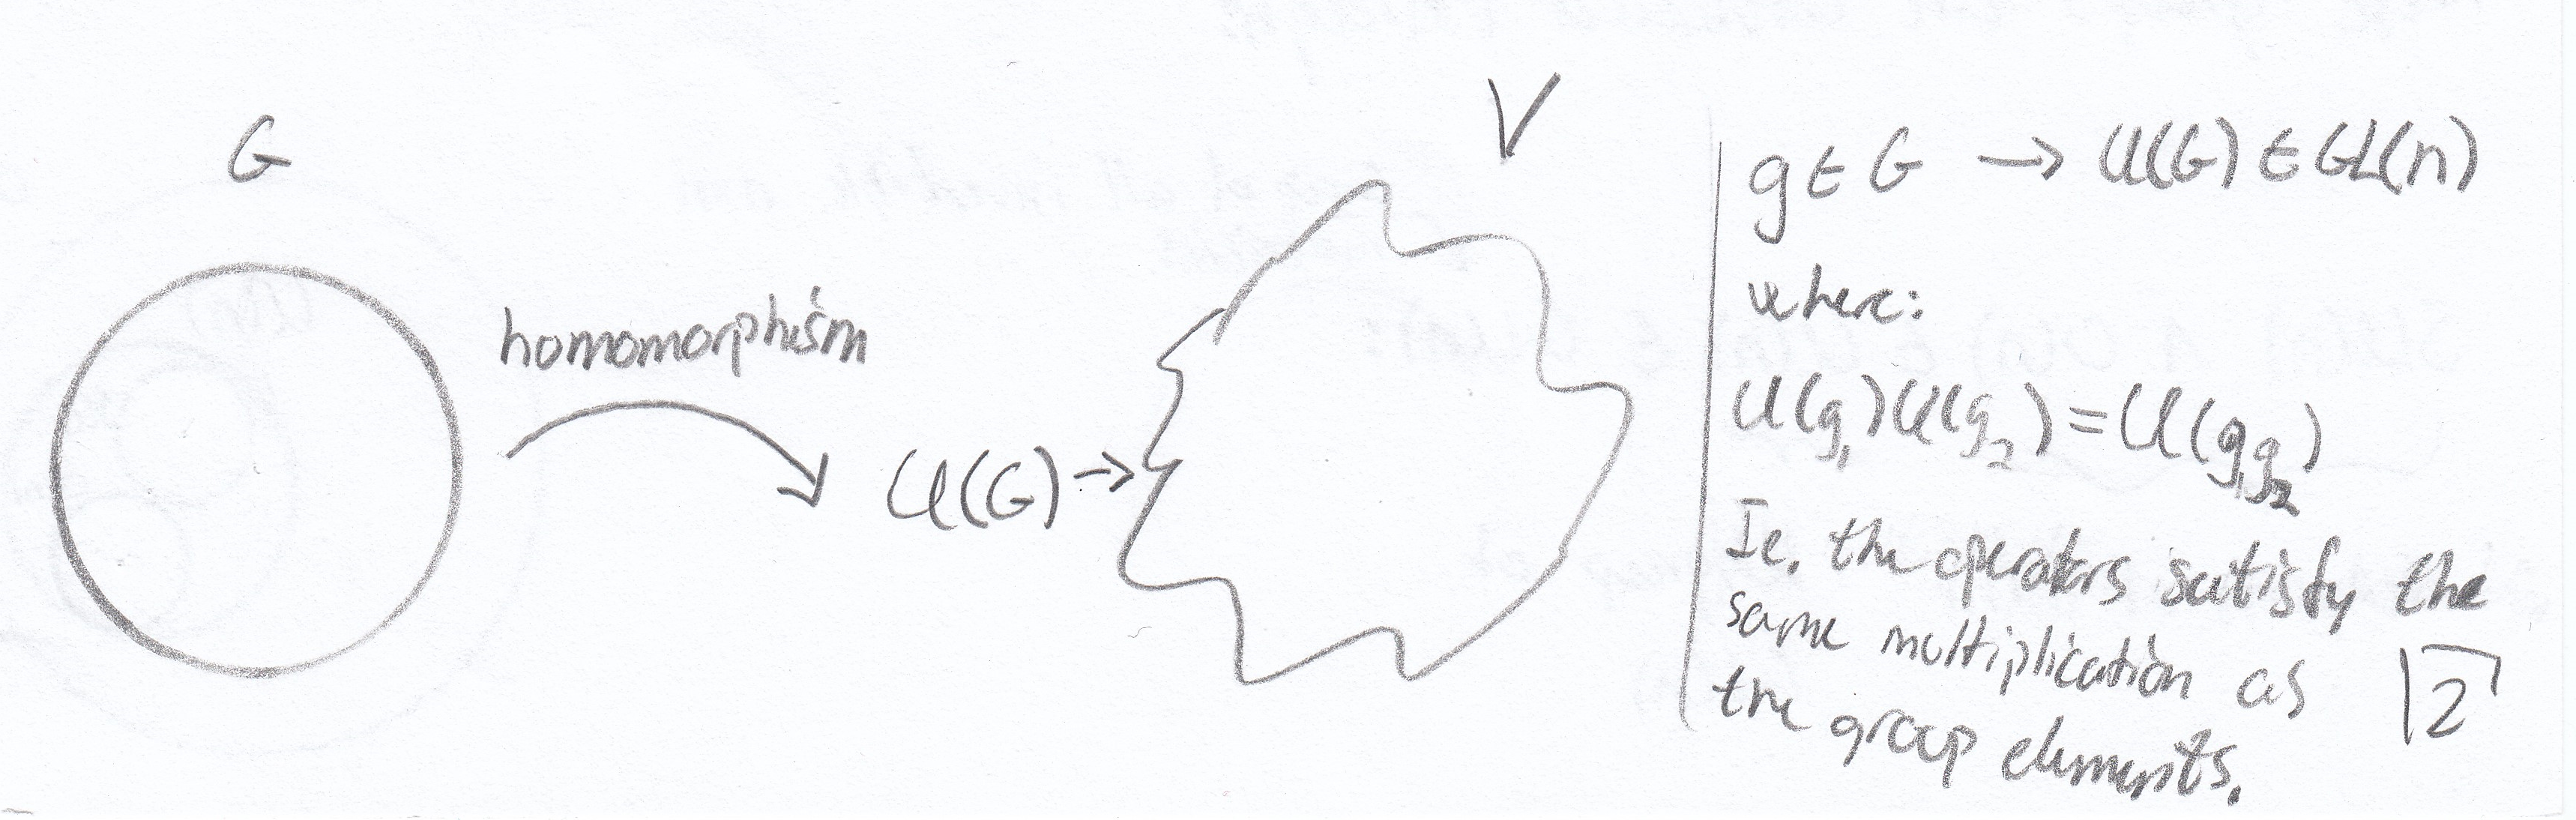
\includegraphics[width=0.6\textwidth]{figures/4}
	\caption{An illustration of a representation of a group.}
	\label{fig:4}
\end{figure} 
In terms of representations of Lie groups it is important to remember that a Lie group is defined in terms of the associated manifold. For this reason one can talk about different representations of groups made up by matrices\footnote{It is a confusing thought to think of representing matrices of a given dimension by other matrices with different dimensions. However, one should think of it like this; a given Lie group has an associated manifold. This manifold can have several representations. For example; $SU(2)$ is the group of $2\times 2$ unitary matrices with unit determinant. The manifold of this group is a circle. The manifold can be represented by either $2\times 2$ matrices or complex number (as is commonly done with the unit circle in complex space).} (eg. $SU(2)$). The representation of a Lie group is a representation of the associated manifold.

\paragraph{Invariant subspace:}\index{invariant subspace} Consider a representation, $U(g)$, of a group, $G$, defined on a linear vector space $V$. $V'\subseteq V$ is called an invariant subspace if for $v\in V'$; $U(g)v\in V'$, $\forall g\in G$. This means that if a vector in the invariant subspace $V'$ act on an arbitrary group element the transformed vector will always be again a part of the invariant subspace, $V'$. For an invariant subspace a representation $U'(g)$ of $G$ on $V'$, called a sub-representation of $U(g)$, can be defined viz
\begin{equation}
	U'(g)v=U(g)v,\quad \forall v\in V'.
\end{equation} 
This leads to the notion that the representation $U(g)$ is not a fundamental but instead composed of smaller building blocks. 

\paragraph{Irreducible representations:} An irreducible representation\index{Irreducible representation} is a representation of a group $G$ on a vector space $V$ that has no invariant subspaces besides $0$ and $V$ itself. Such representations can be thought of as truly fundamental since they are not made up of smaller representations. The irreducible representations of a group are the building blocks from which any other representation of the group can be built. A different approach to irreducible representations can be found by considering similarity transformations\index{Similarity transformation}. Given a matrix, $R$, and an invertible matrix, $S$, the similarity transformation is defined viz
\begin{equation}
	R\Rightarrow R'=S^{-1}RS.
\end{equation} 
If $R$ is a representation of the group $G$, then so is $R'$. An irreducible representation can be defined as a representation that cannot be transformed into block diagonal form via a similarity transformation.  

\paragraph{Generators of a discrete group: }
\index{Generators of a discrete group}
A collection, $c$, of elements of a discrete group, $G$, is said to be generators of the group if multiplication among the generators yield all elements of the group. 
\paragraph{Generators of a continuous group: }
\index{Generators of a continuous group}
In the case of a continuous group the generators are defined different, compared to the discrete group, since there are no single elements in a continuous group, but a continuum of elements. Consider a set of elements, $R$, that depends on some real, continuous parameters
\begin{equation}
	R=R(x,y,z,...).
\end{equation} 
These elements form a continuous group if $R$ fulfil the requirements for a group. If $R$ is differentiable, the group is a Lie group. Differentiability means that $R(dx)$ only differs infinitesimally from $R(0)=e$ by a term od order $dx$. Therefore $R(dx)$ can be parametrized as
\begin{equation}
	R(dx)=e-idxJ,
	\label{dj}
\end{equation} 
where $e$ is the identity element, the "$-i$" is included by convention (to make $J$ Hermitian) and $J$ is \emph{defined} as the generator of the group. By going from $dx\Rightarrow x$
\begin{equation}
	R(x)=\lim\limits_{N\Rightarrow \infty}\bigg(e-i\frac{dxJ}{N}\bigg)^N=e^{-ixJ}.
	\label{eq8}
\end{equation} 
In the considered case, used for illustrative purposes, there is only one parameter ($x$) and one corresponding generator ($J$). In general, a group can have several parameters ($\alpha_i$) and corresponding generators ($t_i$). The different generators make up a vector space. This vectors space is called a Lie algebra. 
\paragraph{Lie algebra:} A Lie algebra is a vector space, $\texttt{g}$, equipped with a binary operation (called the Lie bracket\footnote{The Lie bracket is often called the Lie algebra.}), $[,]: \texttt{g}\times \texttt{g}\Rightarrow \texttt{g}$. The binary operation satisfies the following axioms:
\begin{enumerate}
	\item Bilinearity:$[aX+bY,Z]=a[X,Z]+b[Y,Z]$ and $[Z,aX+bY]=a[Z,X]+b[Z,Y]$, for arbitrary numbers $a,b$ and $\forall X,Y,Z\in \texttt{g}$.
	
	\item Anticommutativity: $[X,Y]=-[Y,X]$ $\forall X,Y\in \texttt{g}$.
	
	\item The Jacobi identity: $[X,[Y,Z]]+[Z,[X,Y]]+[Y,[Z,X]]=0$ $\forall X,Y,Z \in \texttt{g}$. 
\end{enumerate}
The Lie algebra is therefore a vector space consisting of the generators of a Lie group. However, it is important to note that the definition of the Lie algebra makes no reference to any Lie group. Therefore the definition stands on its own and therefore one can talk about different Lie groups having the same Lie algebra. This leads to the definition of a distinguished Lie group.
\paragraph{Distinguished Lie group:} There is precisely one distinguished Lie group for each Lie algebra. The distinguished group has the property of being simply connected. This means that any closed curve on the manifold, corresponding to the Lie group, can be shrunk smoothly to a point. The simply connected group can be thought of as the "mother" of all those groups having the same Lie algebra, because there are maps to all other groups with the same Lie algebra from the simply connected group, but not vice versa. An intuitive name could be the "mother" group of a given Lie algebra. Formally the group is called the \emph{covering group}. All other groups with the same Lie algebra is said to be covered by the simply connected group.

\begin{example}
	Consider the group $SO(2)$. It is a one dimensional group describing rotations in $2$ dimensions. The group is one dimensional since only one continuous parameter, $\theta$, characterizes a rotation. The elements of the group can be represented by $2\times 2$ matrices which commute, and so the group is an abelian group. The group has one generator, $L$, which can be used to generate all elements of the group via
	\begin{equation}
		R(\theta)=e^{-i\theta L}.
	\end{equation} 
	Since the group is designated by $SO(2)$ each matrix is orthogonal an have unit determinant. 
\end{example}
\begin{example}
	This example will consider the isomorphism between $U(1)$ and $SO(2)$. As mentioned in example $4.2$ $SO(2)$ describes rotations in two dimensions and the group elements can be represented, in terms of the generator $L$, as
	\begin{equation}
		R(\theta)=e^{-i\theta L}.
	\end{equation} 
	$U(1)$ is the manifold of unitary $1\times 1$ matrices, i.e. unit complex numbers. The generator of the groups is the identity, $e$, and so the elements can be represented as
	\begin{equation}
		R(x)=e^{-ix}
	\end{equation} 
	There is an isomorphism between the two groups. This can be shown by considering
	\begin{equation}
		R(\theta_1)R(\theta_2)=e^{-i\theta_1 L}e^{-i\theta_2 L}=e^{-i(\theta_1+\theta_2) L}=R(\theta_1+\theta_2),
	\end{equation} 
	\begin{equation}
		f(x_1)f(x_2)=e^{-ix_1}e^{-ix_2}=e^{-i(x_1+x_2)}=f(x_1+x_2).
	\end{equation} 
	It is clear that there is a one-to-one correspondence between $x$ and $\theta$, and so $U(1)$ and $SO(2)$ are isomorphic to each other. The manifold associated with unit complex numbers is the unit circle in the complex plane. Since there is an isomorphism between $U(1)$ and $SO(2)$,the manifold of $SO(2)$ is likewise the unit circle in the complex plane. Hence, one can think of the Lie group as being the unit circle and the manifestation of the elements in complex numbers ($U(1)$) and matrices ($SU(2)$) as representations of the manifold. 
\end{example}


\section{$SO(3)$}
The group $SO(3)$ manifold corresponding to orthogonal $3\times 3$ matrices with unit determinant. The geometric shape of the manifold will be considered in the next section (on $SU(2)$). The reason for this is that $SU(2)$ is the simply connected group of the Lie algebra which it shares with $SO(3)$. Hence, the manifold of $SO(3)$ is a part of the manifold of $SU(2)$.\newline
The matrices describe rotations in $3d$ space. Formally; the $SO(3)$ group consists of all continuous, linear transformations in $3d$ Euclidean space which leave the length of coordinate vectors invariant. The elements of $SO(3)$ does not, in general, commute and so $SO(3)$ is, as opposed to eg. $U(1)$ or $SO(2)$, a non-abelian Lie group.\newline
A generic rotation in $3d$ is parametrized by $3$ rotations, by $3$ continuous angles, around the three coordinate axis. Corresponding to each continuous parameter is a generator, and so $SO(3)$ has $3$ basis generators. The rotations around a given axis form a subgroup of $SO(3)$ that is isomorphic to $SO(2)$. Since there are $3$ coordinate axis' there are $3$ basis generators, denoted by $J_i$. the Lie bracket of the generators is given by
\begin{equation}
	[J^i,J^j]=i\epsilon^{ijk}J^k.
\end{equation} 
From the basis generators a generic element of $SO(3)$ can be described as
\begin{equation}
	R(\alpha,\beta,\gamma)=R_3(\gamma)R_2(\beta)R_1(\alpha)=e^{-iJ_3\gamma}e^{-iJ_2\beta}e^{-iJ_1\alpha},
\end{equation} 
where $\alpha,\beta,\gamma$ are \emph{Euler angles} and the basis matrices $R_i$ are given by
\begin{equation}
	\begin{split}
		&R_1(\alpha)=\begin{bmatrix}
			1 & 0 & 0 \\
			0 & cos(\alpha) & sin(\alpha)\\
			0 & -sin(\alpha) & cos(\alpha)\\
		\end{bmatrix},\\
		& 
		R_2(\beta)=\begin{bmatrix}
			cos(\beta) & 0 & -sin(\beta) \\
			0 & 1 & 0\\
			sin(\beta) & 0 & cos(\beta)\\
		\end{bmatrix},\\
		& 
		R_3(\gamma)=\begin{bmatrix}
			cos(\gamma) & sin(\gamma) & 0 \\
			-sin(\gamma) & cos(\gamma) & 0\\
			0 & 0 & 1\\
		\end{bmatrix},
	\end{split}
	\label{rot}
\end{equation} 
where $R_i$ rotate the coordinate system, not the vector. It is a choice of convention. Rotating the vector is called an active transformation whereas rotating the coordinate system is called a passive transformation. Since the placement of a coordinate system is entirely up to the physicist, i.e. the coordinate system is not a physical thing, it makes more intuitive sense to alternate your definition than actually going in and rotating the physical vector. Hence, here the approach of passive transformations is used.

\section{$SU(2)$}
The group $SU(2)$ is manifold corresponding to unitary $2\times 2$ matrices with unit determinant. The manifold of $SU(2)$ is found by extending the method used to discover the manifold of $SO(2)$. In discovering the manifold of $SO(2)$ it was used that $SO(2)$ is isomorphic to $U(1)$, i.e. sharing manifold, and that $U(1)$ consists of two dimensional complex, unitary numbers which are defined on the unit circle in the complex plane. Extending this analogy the manifold of $SU(2)$ can be found as the manifold of 4 dimensional complex, unitary numbers; quaternions. To describe 4 dimensional complex numbers three imaginary units are needed - As opposed to one imaginary unit for two dimensional complex numbers ($i$). The three imaginary units are defined viz
\begin{equation}
	i^2=j^2=k^2=ijk=-1.
\end{equation} 
Then a 4 dimensional complex number, a quaternion, can be parametrized viz
\begin{equation}
	q=a+bi+cj+dk.
\end{equation} 
The set of unit quaternions are those that satisfy
\begin{equation}
	qq^\dagger=a^2+b^2+c^2+d^2=1.
\end{equation} 
Just as complex numbers can be represented as matrices by mapping the complex unit ($i$) to a matrix, so can quaternions. Specifically~\citep{Schwichtenberg2015}
\begin{equation}
	I=\begin{bmatrix}
		1 & 0\\
		0 & 1\\
	\end{bmatrix}, \quad \hat{i}=\begin{bmatrix}
		i & 0 \\
		0 & -i \\
	\end{bmatrix}, \quad \hat{j}=\begin{bmatrix}
		0 & 1\\
		-1 & 0 \\
	\end{bmatrix}, \quad \hat{k}=\begin{bmatrix}
		0 & i \\
		i & 0 \\
	\end{bmatrix}.
\end{equation} 
This means the generic quaternion can be parametrized viz
\begin{equation}
	q=aI+b\hat{i}+c\hat{j}+d\hat{k}=\begin{bmatrix}
		a+ib & c+id\\
		-c+id & a-ib\\
	\end{bmatrix}\Rightarrow det(q)=a^2+b^2+c^2+d^2.
	\label{as}
\end{equation} 
Comparing equation \eqref{as} to the definition of unit quaternions ($qq^\dagger=1$), it is clear that the matrices must be unitary and have unit determinant. That is the matrices make up the group $SU(2)$. Hence, unit quaternions are isomorphic to $SU(2)$ just like $U(1)$ is isomorphic to $SO(2)$. Hence, the manifold of $SU(2)$ can be described by the unit quaternions. The unit quaternions are characterized by $a^2+b^2+c^2+d^2=1$, analogous to how 2 dimensional unit complex numbers are characterized by $z=a+ib\Rightarrow a^2+b^2=1$. $a^2+b^2=1$ describes the unit circle, $S^1$. Hence, the manifold of two dimensional unit complex numbers is the unit circle in the complex plane. Likewise $a^2+b^2+c^2+d^2=1$ describes the unit three sphere, $S^3$. Hence, the manifold of four dimensional unit complex numbers is the unit three sphere. The unit three sphere is a simply connected manifold. Hence, $SU(2)$ is simply connected.

\subsection{Relationship between $SO(3)$ and $SU(2)$}
To relate the two groups it will be investigated how quaternions can be used to rotate a vector. Parametrizing a vector viz
\begin{equation}
	v=v_x\hat{i}+v_y\hat{j}+v_z\hat{k}=\begin{bmatrix}
		iv_x & v_y+iv_z\\
		-v_y+iv_z & -iv_x\\
	\end{bmatrix}\Rightarrow det(v)=x^2+y^2+z^2.
	\label{as4}
\end{equation} 
The determinant of $v$ is the length of the vector. Since the length of a vector is conserved during a rotation, the transformation must preserve determinants. This means restricting ourselves to unit quaternions as a means to transform the vector
\begin{equation}
	v\Rightarrow v'=q^{-1}vq,
	\label{as1}
\end{equation} 
where once again the approach of passive transformations has been applied. The inverse transformation, $qvq^{-1}$, is the corresponding active rotation\footnote{$qvq^{-1}$ is just a the inverse transformation of $q^{-1}vq$. This makes intuitively sense since rotating a vector in one direction is equivalent to rotating the coordinate system in the opposite direction. Hence, the definition of active and passive rotations is related to the definition of positive and negative angles also.}. In order to relate the transformation of equation \eqref{as1} to rotations the rotation angles must be introduced. In this regard it is convenient to parametrize the unit quaternion viz
\begin{equation}
	q=cos(\theta)+sin(\theta)||\vec{e}||,
\end{equation} 
where $||\vec{e}||$ is the normalized rotation axis. For transparency consider a rotation of $\frac{\vec{x}}{|\vec{x}|}\equiv \hat{x}$ around the $z$-axis. In this case
\begin{equation}
	q=cos(\theta)I+sin(\theta)k=\begin{bmatrix}
		cos(\theta) & isin(\theta)\\
		isin(\theta) & cos(\theta)\\
	\end{bmatrix}.
	\label{as2}
\end{equation} 
Using equation \eqref{as2}
\begin{equation}
	q^{-1}\hat{i}q=\begin{bmatrix}
		cos(\theta) & -isin(\theta)\\
		-isin(\theta) & cos(\theta)\\
	\end{bmatrix}\begin{bmatrix}
		i & 0\\
		0& -i\\
	\end{bmatrix}\begin{bmatrix}
		cos(\theta) & isin(\theta)\\
		isin(\theta) & cos(\theta)\\
	\end{bmatrix}=\begin{bmatrix}
		icos(2\gamma) & -sin(2\theta)\\
		sin(2\theta) & -icos(2\theta)\\
	\end{bmatrix}.
	\label{as3}
\end{equation} 
Comparing equation \eqref{as3} to equation \eqref{as4}
\begin{equation}
	\begin{split}
		&v_x\Rightarrow v'_x=cos(2\theta),\\
		&v_y\Rightarrow v'_y=-sin(2\theta),\\
		&v_z\Rightarrow v'_z=0.\\
	\end{split}
	\label{as5}
\end{equation} 
Rotating a vector in 3-space reveals, cf. equation \eqref{rot}
\begin{equation}
	R_3(\gamma)\hat{x}
	\begin{bmatrix}
		cos(\gamma) & sin(\gamma) & 0 \\
		-sin(\gamma) & cos(\gamma) & 0\\
		0 & 0 & 1\\
	\end{bmatrix}\begin{bmatrix}
		1\\0 \\0\\
	\end{bmatrix}=\begin{bmatrix}
		cos(\gamma)\\
		-sin(\gamma)\\
		0\\
	\end{bmatrix}.
	\label{as6}
\end{equation} 
By comparing equation \eqref{as5} and \eqref{as6} it is clear that $\gamma=2\theta$. That is, in rotating $\hat{x}$ by $\theta$ the vector is rotated by $2\gamma$ in 3-space. This means that there is a two-to-one map from the manifold of $SU(2)$ to the manifold of $SO(3)$, i.e. there are two elements in the manifold of $SU(2)$ that corresponds to the same element in the manifold of $SO(3)$. Hence given one element of the manifold of $SU(2)$ one can find the corresponding element in the manifold of $SO(3)$ but not vice versa. this confirms that the manifold of $SU(2)$ is indeed simply connected. Since there is a two-to-one correspondence between the manifolds of $SU(2)$ and $SO(3)$, and the manifold of $SU(2)$ is the unit three sphere, the manifold of $SO(3)$ must be half a unit three sphere. Since the manifold of $SU(2)$ covers the manifold of $SO(3)$ twice it is called the double cover of the manifold of $SO(3)$.

\section{The Lorentz group}
\label{sec:lor}
The Lorentz group\index{The Lorentz group}, denoted by\footnote{Three space-like dimensions and one time-like dimension.} $O(3,1)$, is the group representing the coordinate transformations of $SR$; boosts and rotations that is. Because the Lorentz group describes the transformations of SR, which are transformations of four vectors, the Lorentz groups is often analysed in a certain representation; the vector representation. In the vector representation an event in SR is described by a four vector on the form
\begin{equation}
	x^\mu\equiv \begin{bmatrix}
		t \\
		\vec{x}\\
	\end{bmatrix}.
\end{equation} 
This vector is called contravariant (index up) and it is defined by its transformation properties
\begin{equation}
	dx^\mu\Rightarrow d{x'}^\mu=\underbrace{\frac{\partial {x'}^\mu}{\partial x^\nu}}_{\Lambda^\mu_{\,\,\,\nu}}dx^\nu.
	\label{contra}
\end{equation} 
Any vector that transforms in this way is called a contravariant vector. Likewise, a covariant vector is defined by
\begin{equation}
	dx_\mu\Rightarrow d{x'}_\mu=\underbrace{\frac{\partial {x'}_\mu}{\partial x_\nu}}_{(\Lambda^{-1})^\nu_{\,\,\,\mu}=\Lambda_\mu^{\,\,\,\nu}}dx_\nu.
\end{equation} 
The contra-variant and covariant vectors are related by the metric via
\begin{equation}
	x^\mu=g^{\mu\nu}x_\nu.
\end{equation} 
During the coordinate transformations, the length of the vectors, $x^\mu x_\mu\equiv x\cdot x=x^2$, is invariant. The length of a vector can be expressed via the metric
\begin{equation}
	x^\mu x_\mu=g_{\mu\nu}x^\mu x^\nu=g_{\mu\nu}x'^\mu x'^\nu=g_{\mu\nu}\Lambda^\nu_{\,\,\,\,\alpha}\Lambda^\mu_{\,\,\,\,\beta}x^\alpha x^\beta.
\end{equation} 
Rearranging the dummy indices
\begin{equation}
	g_{\mu\nu}x^\mu x^\nu=g_{\alpha\beta}\Lambda^\alpha_{\,\,\,\nu}\Lambda^\beta_{\,\,\,\mu}x^\nu x^\mu\Rightarrow g_{\mu\nu}=g_{\alpha\beta}\Lambda^\alpha_{\,\,\,\nu}\Lambda^\beta_{\,\,\,\mu},
\end{equation} 
which can be written $g=\Lambda^Tg\Lambda$ in matrix notation. Taking the determinant, and using that $g_{\mu\nu}=\eta_{\mu\nu}=diag(1,-1,-1,-1)$ for Minkowski space
\begin{equation}
	det(\eta)=det(\Lambda^T)det(\eta)det(\Lambda)\Rightarrow det(\Lambda^T)det(\Lambda)=1.
\end{equation} 
Use now that $det(\Lambda^T)=det(\Lambda)$ to find $det(\Lambda)^2=1\Rightarrow det(\Lambda)=\pm 1$. Transformations for which $det(\Lambda)= 1$ are called proper. Transformations for which $det(\Lambda)= -1$ are called improper. Another classification comes from
\begin{equation}
	g_{00}=1=\Lambda^\alpha_{\,\,\,0}\Lambda^\beta_{\,\,\,0}g_{\alpha\beta}=(\Lambda^0_{\,\,\,0})^2-\sum_{i=1}^{3}(\Lambda^i_{\,\,\,0})^2\Rightarrow |\Lambda^0_{\,\,\,0}|>1.
\end{equation} 
This allows $\Lambda^0_{\,\,\,0}>1$ or $\Lambda^0_{\,\,\,0}<-1$. The transformations characterized by $\Lambda^0_{\,\,\,0}>1$ are called orthochronous whereas transformations characterized by $\Lambda^0_{\,\,\,0}<-1$ are called non-orthochronous. Hence, the Lorentz transformations can be grouped into $4$ categories\footnote{That this is correct can be seen by considering the $TP\Lambda^{po}$-term; the determinant must be positive since it is proper. The determinant of $\Lambda^{po}$ is defined as positive and since the determinant is distributive and negative for both $T,P$, the table must be as shown. The table is confirmed by \citet{Srednicki2027}.} shown in figure \ref{fig:5}.
\begin{figure}[H]
	\captionsetup{width=1\textwidth}
	\centering
	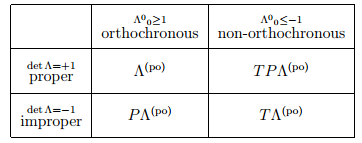
\includegraphics[width=0.4\textwidth]{figures/5}
	\caption{The different categories of Lorentz transformations.}
	\label{fig:5}
\end{figure} 
As shown in figure \ref{fig:5} the different elements of the categories can all be expressed in terms of proper, orthochronous transformations followed by a time-inversion and/or parity operation. Parity is called the "mirror-transformation". Until 1956 physicists believed all physical systems should be invariant under parity. However, in 1956 it was found that the weak interaction violates parity. Mathematically, parity is expressed viz
\begin{equation}
	\Lambda_P x=\begin{bmatrix}
		t\\
		-\vec{x}\\
	\end{bmatrix}, \quad \text{and} \quad  \Lambda_Pp=\begin{bmatrix}
		p^0\\
		-\vec{p}\\
	\end{bmatrix},
\end{equation} 
where $\Lambda_P=diag(1,-1,-1,-1)$ in the vector representation\footnote{Not in general, only in the vector representation.}. Similarly, time-inversion is given by
\begin{equation}
	\Lambda_T x=\begin{bmatrix}
		-t\\
		\vec{x}\\
	\end{bmatrix}, \quad \text{and} \quad  \Lambda_Tp=\begin{bmatrix}
		-p^0\\
		\vec{p}\\
	\end{bmatrix},
\end{equation} 
where $\Lambda_T=diag(-1,1,1,1)$ in the vector representation\footnote{Not in general, only in the vector representation.}. Since the subsets that are not elements of the proper orthochronous subgroup can be determined via applying parity and/or time-inversion, the elements of the proper, orthochronous subgroup is of special interest. Since all elements of the Lorentz group is enclosed in $O(3,1)$, and proper means $det(\Lambda)=1$, the proper, orthochronous transformations (indeed all proper transformations) are members of $SO(3,1)$- in this case a subgroup of $O(3,1)$. $SO(3,1)$ is also called the proper Lorentz group, but most often it is just referred to as the Lorentz group. $SO(3)$ consists of all boost, rotations and combinations of the two. A generic element of the proper, orthochronous subgroup of the Lorentz group can therefore be expressed as
\begin{equation}
	\Lambda^\mu_{\,\,\,\nu}=\Lambda(R')^\mu_{\,\,\,\alpha}\Lambda(\gamma)^\alpha_{\,\,\,\beta}\Lambda(R)^\beta_{\,\,\,\nu}.
\end{equation} 
The $\Lambda$-matrices form a representation of the Lorentz group.

\begin{example}
	\index{4-vector}
	\index{Current density}
	\index{Four current}	
	\emph{Prove that $J^\mu$ is a $4$-vector, where}\newline
	\begin{equation}
		J^\mu=\begin{bmatrix}
			\rho\\
			J_x\\
			J_y\\
			J_z\\
		\end{bmatrix}=\begin{bmatrix}
			\rho\\
			\rho v_x\\
			\rho v_y\\
			\rho v_z\\
		\end{bmatrix}=\begin{bmatrix}
			\rho\\
			\vec{J}\\
		\end{bmatrix}.
	\end{equation} 
	An $n$-dimensional vector is a physical object that can be represented as a $n\times1$ matrix. Because a vector can be represented as a matrix, it must obey the rules of linear algebra, including scalar multiplication, vector addition, dot product, scalar and vector projections. Further more a vector is a rank 1 tensor, which means that it must transform in a well defined way during a coordinate transformation; it must conserve its length during a coordinate transformation. This last definition will be used to verify that $J^\mu$ is in fact a 4-vector. For a $4$-vector the length is called the spacetime interval ($ds^2$). Consider a volume ($V_1$) of charge moving with a uniform velocity ($v_{1x}$) as observed from the reference frame $S_1$\footnote{I only consider movement along the $x$-axis to illustrate the principle. A general treatment is rather cumbersome.}. In this frame the spacetime interval will be given by
	\begin{equation}
		ds_1^2=\rho_1^2(v_{1x}^2-1),
	\end{equation} 
	where the $y$ and $z$ components of the velocity is zero and the subscript on $ds_1$ is introduced because current density has not been proven a $4$-vector yet (and therefore that $ds$ for different reference frames is the same). From $S_1$ the volume containing the charge is contracted via.
	\begin{equation}
		V_1=\gamma^{-1}(v_{1x})V_0,
	\end{equation} 
	where $\gamma=\gamma(v)=(1-v^2)^{-\frac{1}{2}}$. The volume is contracted in the direction parallel to the direction of motion, and hence the volume is diminished as seen from $S_1$. Considering the scenario from the reference frame of $S_2$, which moves with a uniform velocity $v$ with respect to $S_1$ and parallel to the $x$-axis of $S_1$, the volume is seen to be moving with $v_{2x}$. Here the volume is observed to be
	\begin{equation}
		V_2=\gamma^{-1}(v_{2x})V_0.
	\end{equation} 
	Using that
	\begin{equation}
		v_{2x}=\frac{v_{1x}-v}{1-vv_{1x}}.
	\end{equation} 
	The volumes in the two reference frames can be related in terms of the velocity in one reference frame. For example
	\begin{equation}
		\frac{V_1}{V_2}=\gamma(v)(1-vv_{1x}).
	\end{equation} 
	This relation can be used to determine how the charge density transforms. There must be conservation of charge ($Q=\rho_iV_i$) between reference frames. Therefore
	\begin{equation}
		V_1\rho_1=V_2\rho_2\Rightarrow \rho_2=\rho_1\frac{V_1}{V_2}=\rho_1\gamma(v)(1-vv_{1x}).
	\end{equation} 
	Using this to express $ds_2^2$
	\begin{equation}
		ds_2^2=\rho_2^2(v_{2x}^2-1)=\bigg(\rho_1\gamma(v)(1-vv_{1x})\bigg)^2\bigg(\bigg(\frac{v_{1x}-v}{1-vv_{1x}}\bigg)^2-1\bigg)=\rho_1^2(v_{1x}^2-1)=ds_1^2.
	\end{equation} 
	The space time interval is conserved ($ds_1=ds_2$), and $J^\mu$ is therefore a $4$-vector. One can also say that $\rho$, as has been shown for the $x$-component, transforms via the Lorentz-transformation and therefore the length of the $4$-vector transforms from reference frame to reference frame via
	\begin{equation}
		J'^\mu J_\mu'={\Lambda_x}(v)^\mu_\nu {\Lambda^{-1}_x}(v)^\nu_\mu J^\nu J_\nu=J^\nu J_\nu,
	\end{equation} 
	where $L$ is the Lorentz matrix
	\begin{equation}
		\Lambda_x(v)=\begin{bmatrix}
			\gamma & -v\gamma & 0 & 0\\
			-v \gamma & \gamma & 0 & 0\\
			0 & 0 & 1 & 0\\
			0 & 0 & 0 & 1
		\end{bmatrix}.
	\end{equation} 
	As is apparent the length of the vector is conserved as it should be in order for $J^{\mu}$ to be a vector.
\end{example}


\begin{example}
	\emph{A spaceship travels with a velocity, $\vec{v}^T=\frac{1}{2}\begin{bmatrix}
			1 & 1 & 1\\
		\end{bmatrix}$, when it is hit by a cosmic ray carrying a four momentum, $p^T=\begin{bmatrix}
			300 & 299 & 0& 0\\
		\end{bmatrix}\cdot10^{-27}kg$.}
	\begin{figure}[H]
		\captionsetup{width=1\textwidth}
		\centering
		\includegraphics[width=0.6\textwidth]{billeder/ss}
		\caption{The scenario with the three reference frames involved.}
		\label{fig:ss}
	\end{figure} 
	\begin{enumerate}
		\item \emph{Find the four velocity, $u$, of the spaceship.}
		
		From $S$
		\begin{equation}
			u=\gamma(v)\begin{bmatrix}
				1 \\
				\vec{v}\\
			\end{bmatrix}=\begin{bmatrix}
				2 \\
				2\vec{v}\\
			\end{bmatrix},
		\end{equation} 
		where $v=|\vec{v}|$.
		
		\item \emph{Find the energy of the cosmic ray in $S'$.}
		
		I know the energy in $S$ from $p$, so I will create a Lorentz transformation to transform $p$ from $S$ to $S'$. To this end I will use a general Lorentz transformation which will consist of two rotations, one boost and the inverse rotations. The idea is to rotate the coordinate-system so it aligns with the velocity of the space-ship, boost so the coordinate system, in rotated form, moved with the spaceships, and lastly rotate the coordinate system back. The result will be a boost of $S$ such that is follows the spaceship, i.e. $S\Rightarrow S'$. First, I will rotate (counter clockwise, i.e. positive angle) around the $z$-axis such that the $\vec{v}$lies in the $zx$ plane. Hereafter I will rotate (clockwise, i.e. negative angle) around the (new, since I have rotated around the $z$-axis) $y$-axis such that the $x$-axis is aligned with $\vec{v}$. Hereafter I will boost along the $x$-axis and rotate back. The Lorentz transformation
		\begin{equation}
			\Lambda_{tot}=\big(\Lambda(R_y(\theta_2))\Lambda(R_z(\theta_1))\big)^{-1}\Lambda_x(\gamma(v))\Lambda(R_y(\theta_2))\Lambda(R_z(\theta_1),
		\end{equation} 
		where
		\begin{equation}
			\Lambda(R_i(\theta_j))=\begin{bmatrix}
				1 & 0 & 0 & 0\\
				0 &   &   &   \\
				0 &   & R_i(\theta_j) & \\
				0 &   &   & \\
			\end{bmatrix}, \quad \Lambda_x(\gamma(v))=\begin{bmatrix}
				\gamma(v)&-v\gamma(v)&0&0\\
				-v\gamma(v)&\gamma(v)&0&0\\
				0&0&1&0\\
				0&0&0&1\\
			\end{bmatrix}.
		\end{equation} 
		Since I know $v$, all I need is the two rotation angles. I find these by considering the criterion for each rotation. After the first rotation the velocity should be in the $zx$-plane, and therefore the transformed velocity should have no $y$-component. Hence, I can find the first rotation angle from
		\begin{equation}
			\begin{split}
				R_z(\theta_1)\vec{v}&\propto\begin{bmatrix}
					cos(\theta_1) & sin(\theta_1) & 0 \\
					-sin(\theta_1) & cos(\theta) & 0 \\
					0 & 0 & 1 \\
				\end{bmatrix}\begin{bmatrix}
					1\\
					1\\
					1\\
				\end{bmatrix}\\
				&=\begin{bmatrix}
					cos(\theta_1)+sin(\theta_1)\\
					sin(\theta_1)-cos(\theta_1)\\
					1\\
				\end{bmatrix}\\
				&= \begin{bmatrix}
					\dots\\
					0\\
					1\\
				\end{bmatrix}.\\
			\end{split}
		\end{equation} 
		In order for the second component of the transformed velocity to vanish $sin(\theta_1)=cos(\theta_1)\Rightarrow \theta_1=\frac{\pi}{4}$. From the second rotation the $x$-axis is to align with $\vec{v}$, so the third component of the transformed velocity is to vanish. Hence, I can find the second rotation angle from
		\begin{equation}
			\begin{split}
				R_y(\theta_2)R_z(\theta_1)\vec{v}&\propto
				\begin{bmatrix}
					cos(\theta_2) & 0 & -sin(\theta_2) \\
					0 & 1 & 0 \\
					sin(\theta_2) & 0 & cos(\theta_2) \\
				\end{bmatrix}\begin{bmatrix}
					\sqrt{2}\\
					0\\
					1\\
				\end{bmatrix}\\
				&=\begin{bmatrix}
					\sqrt{2}cos(\theta_2)-sin(\theta_2)\\
					0\\
					cos(\theta_2)+\sqrt{2}sin(\theta_2)\\
				\end{bmatrix}\\
				&=\begin{bmatrix}
					|\vec{v}|\\
					0\\
					0\\
				\end{bmatrix}.\\
			\end{split}
		\end{equation} 
		In order for the third component of the transformed velocity to vanish; $cos(\theta_2)+\sqrt{2}sin(\theta_2)=0\Rightarrow \theta_2=-35.264 deg$. By using the two rotation angles I can now transform $p$ and find it in $S'$
		\begin{equation}
			p'=\Lambda_{tot}p=\begin{bmatrix}
				301 \\
				296/3\\
				-601/3\\
				-601/3\\
			\end{bmatrix}\cdot 10^{-27}kg.
		\end{equation} 
		Hence, the energy (now in SI units) as seen from $S'$ is $301\cdot 10^{-27}kg\cdot c^2\simeq 2.7\cdot 10^{-8}J$.
		
		\item \emph{Calculate the energy in $S'$ from $-g_{\mu\nu}u^\mu p^\nu$. Why does this work?}
		
		I can also calculate the energy from $-g_{\mu\nu}u^\mu p^\nu$. $-g_{\mu\nu}u^\mu p^\nu$ has all indices contracted and so is a Lorentz scalar. In the rest frame of the spaceship $u^T=\begin{bmatrix}
			1 \\\vec{0}\\
		\end{bmatrix}$ and so it works to pick out the zeroth component of the momentum vector; the energy. So, the quantity is the energy in $S'$ and it is invariant between reference frame. Hence, I can calculate it in $S$ and thereby obtain the energy in $S'$. I find
		\begin{equation}
			\begin{split}
				-g_{\mu\nu}u^\mu p^\nu&=u^0p^0-u^1p^1-u^2p^2-u^3p^3\\
				&=(2\cdot 300-299)\cdot 10^{-27}kg\cdot c^2\\
				&=301\cdot 10^{-27}kg\cdot c^2.
			\end{split}
		\end{equation} 
	\end{enumerate}
\end{example}

\section{The Poincare' group}
The Poincare' group, $ISO(1,3)$, is the group of Lorentz transformations and translations. The Poincare' group encompasses the transformations the physical theories, in the absence of general relativistic effects, should obey, i.e. the physical theory should be invariant under translation, rotation and boosts - Physical theories should be invariant under Poincare' transformations. A generic Poincare' transformation is on the form
\begin{equation}
	x^\mu\Rightarrow {x'}^\mu=\Lambda^{\mu}_{\,\,\, \nu}x^\nu+a^{\mu}.
\end{equation}  
where $a^\mu$ is a constant four vector. From which it is clear that the Poincare' group contains Lorentz transformations and translations. The generators of the Poincare' group are the generators of the Lorentz group, $J_i,K_i$ and the generator of translation in flat space-time (Minkowski space); $p^\mu$. In terms of the generators, the algebra reads
\begin{equation}
	\begin{split}
		&[J_i,J_j]=i\epsilon_{ijk}J_k, \quad [J_i,K_j]=i \epsilon_{ijk}K_k, \quad [K_i,K_j]=-i\epsilon_{ijk}J_k,\\
		&[J_i,p_j]=i\epsilon_{ijk}p_k,\quad [j_i,p_0]=0,\quad [k_i,p_j]=i\delta_{ij}p_0,\quad [k_i,p_0]=-ip_i.
	\end{split}
\end{equation} 
